% Canonical discussion manuscript using the verified ICLR 2027 template.
% The nine-page initial-submission limit is pinned in template_manifest.json.
\documentclass{article}
\usepackage{iclr2027_conference,times}
\usepackage{microtype,graphicx,booktabs,array}
\usepackage{xurl}
\usepackage{hyperref}
% Discussion-copy label only: retain the pinned upstream style unchanged.
% Fail visibly if the reviewed template changes either anonymous-copy label.
\usepackage{etoolbox}
\makeatletter
\patchcmd{\@maketitle}
  {Under review as a conference paper at ICLR 2027}
  {Discussion draft. Not submitted.}
  {}{\PackageError{tikitorch}{ICLR running-head label changed}{Review the pinned template before sharing.}}
\patchcmd{\@maketitle}
  {Paper under double-blind review}
  {Discussion draft. Not submitted.}
  {}{\PackageError{tikitorch}{ICLR title-page label changed}{Review the pinned template before sharing.}}
\makeatother
\usepackage{amsmath,amssymb,amsthm,mathtools}
\usepackage{tikz}
\usetikzlibrary{arrows.meta,positioning}
\usepackage{placeins}
\theoremstyle{plain}
\newtheorem{theorem}{Theorem}[section]
\newtheorem{proposition}[theorem]{Proposition}
\newtheorem{lemma}[theorem]{Lemma}
\newtheorem{corollary}[theorem]{Corollary}
\theoremstyle{definition}
\newtheorem{definition}[theorem]{Definition}
\newtheorem{assumption}[theorem]{Assumption}
\theoremstyle{remark}
\newtheorem{remark}[theorem]{Remark}
\newcommand{\R}{\mathbb{R}}
\newcommand{\VJP}{\operatorname{VJP}}
\newcommand{\cert}{\mathcal{C}}
\newcommand{\ttorch}{\textsc{TikiTorch}}
\newcommand{\code}[1]{\texttt{#1}}
\newcolumntype{L}[1]{>{\raggedright\arraybackslash}p{#1}}
\title{TikiTorch: Learning with\\Additive Hard Routing}
\author{Anonymous Authors}
\hypersetup{colorlinks=true,allcolors=blue,pdfauthor={},pdftitle={TikiTorch: Learning with Additive Hard Routing},pdfsubject={TikiTorch discussion draft; not submitted}}

\begin{document}
\maketitle

\begin{abstract}
Additive hard routing changes what a neural network needs to retain for
learning. In an additive tropical layer, each output selects a candidate
$x_i+w_i$. Once that winner is known, backpropagation sends the incoming
gradient to the selected input and weight: it needs their addresses, not
their forward values. Hard selection therefore turns this layer's backward
computation into routing and accumulation. We present \ttorch{}, a PyTorch
companion that makes this property usable across an integrated library of
tropical operators, layers, models, differentiation tools, and backends.
We characterize when discrete routes suffice for both activation and
parameter gradients, show how the property composes, and implement packed
device-resident route tapes within ordinary first-order autograd.
The resulting design separates the state needed to learn from the values
needed to run the forward pass. On three source-snapshotted MorphSSM
configurations, the retained device-tape payload is
2.04--2.98$\times$ smaller than a specified layer/embedding checkpoint
boundary set. These measurements establish a compact backward representation,
not yet lower peak memory or cheaper learning at matched task quality.
\ttorch{} provides the software and experimental interfaces needed to test
that next step, while keeping losses, optimizers, and other non-route
boundaries explicit.
\end{abstract}

\section{Introduction}

The cost of learning is not just the cost of prediction. Backpropagation
also needs information from the forward pass, often retained as activations
or recovered through recomputation. This creates a practical question for
resource-constrained learning: \emph{can we choose operators whose gradients
need less information in the first place?} Such a choice could let useful
models train with longer contexts, larger batches, or smaller hardware.
It need not make every forward operation cheaper to be valuable.

Additive tropical, or morphological, layers offer a particularly direct
answer \citep{ritter1996morphological,franchi2020morphological}. Instead of a
sum of products, consider $y_j=\max_i(x_i+w_{ji})$. Away from a tie, the
winning candidate is locally an addition. Its derivatives with respect to
the selected input and weight are both one, and all unselected derivatives
are zero. Backward therefore follows the recorded winners and accumulates
gradients. In contrast, a dense layer $y=Wx$ has weight gradient $qx^T$:
even knowing which dense expert was selected does not remove the input
values from the parameter update.

The useful simplification is thus in the \emph{derivative graph}: for
additive hard-selected extrema, activation-valued derivative coefficients
are replaced by discrete routes. Finding those routes still requires the
forward comparisons. This is not a claim that hard routing automatically
makes the forward sparse, or that any sparsely activated architecture can
discard its activations. It is a consequence of the combination of
\emph{hard selection and additive parameterization}.

\ttorch{} turns that mathematical structure into a research platform built
on PyTorch \citep{paszke2019pytorch}. A useful platform needs more than an
isolated max-plus kernel: researchers need composable layers and models,
correct gradients through shared operations, compact route recording,
interoperability with task losses and optimizers, and measurements of the
complete training step. \ttorch{} connects these pieces so that operator
choices can be studied jointly with their learning dynamics and systems
costs. Its general-purpose tropical library is broader than its current
route-tape adapter; support for each optimized training path is explicit.

We make three contributions:
\begin{enumerate}
\item \textbf{A precise explanation of the simplification.} We characterize
when routes determine both input and trainable-parameter gradients, and
show how these local rules compose without recovering internal activations.
Explicit tie rules and counterexamples delimit the result.
\item \textbf{A library that exploits it.} Tropical operators, neural-network
modules and model families connect to streamed, packed route tapes,
first-order PyTorch autograd, pluggable backends, and training-recipe audits.
The implementation exposes both the optimized subset and its boundaries.
\item \textbf{An executable evaluation path.} Correctness checks and
source-bound retained-state measurements establish the measured
representation benefit. A full-step comparison protocol makes the remaining
question---useful learning at lower total resource cost---testable.
\end{enumerate}

Morphological backpropagation already exploits active paths
\citep{groenendijk2023geometric}, and compact backward encodings have a long
history \citep{jain2018gist}. Our contribution is not a new chain rule.
It is an explicit, compositional account of the required learning state,
realized in a library that lets researchers build, train, and compare the
corresponding models. Arithmetic audits and historical FPGA experiments
provide a further path toward specialized hardware, rather than a
prerequisite for the training-state opportunity.

\begin{figure*}[t]
\centering
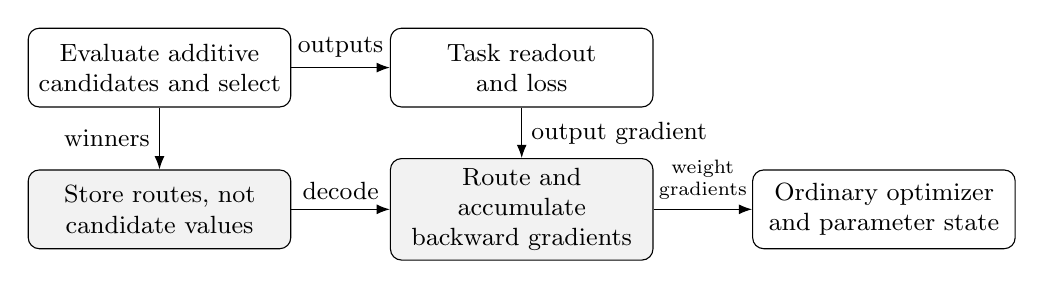
\begin{tikzpicture}[>=Latex, every node/.style={font=\small},
 box/.style={draw,rounded corners,align=center,minimum height=10mm,text width=31mm}]
\node[box] (forward) at (0,0) {Evaluate additive\\candidates and select};
\node[box] (boundary) at (4.6,0) {Task readout\\and loss};
\node[box] (update) at (9.2,-1.8) {Ordinary optimizer\\and parameter state};
\node[box,fill=black!5] (tape) at (0,-1.8) {Store routes, not\\candidate values};
\node[box,fill=black!5] (reverse) at (4.6,-1.8) {Route and accumulate\\backward gradients};
\draw[->] (forward) -- node[above] {outputs} (boundary);
\draw[->] (forward) -- node[left] {winners} (tape);
\draw[->] (tape) -- node[above] {decode} (reverse);
\draw[->] (boundary) -- node[right] {output gradient} (reverse);
\draw[->] (reverse) -- node[above,align=center,font=\scriptsize] {weight\\gradients} (update);
\end{tikzpicture}
\caption{What additive hard routing buys. The forward still evaluates
candidates, but the shaded backward path uses winner addresses instead of
their activation values. A supported composite model also records any
required auxiliary fields, such as normalization exponents. The task
boundary and optimizer retain their own state; they need not be tropical or
multiplier-free to benefit from a route-trained body.}
\label{fig:contracts}
\end{figure*}

\section{From Forward Values to Backward Routes}
\label{sec:contract}

\subsection{A Winner Determines Two Gradients}

Consider $y=\max(x_1+w_1,x_2+w_2,x_3+w_3)$ and suppose the second
candidate wins. Locally, $y=x_2+w_2$. For an incoming gradient
$q=\partial\mathcal{L}/\partial y$, the selected backward rule is simply
\begin{equation}
 \bar x=(0,q,0),\qquad \bar w=(0,q,0).
 \label{eq:worked-route}
\end{equation}
The same result holds for any forward values that produce that winner.
Saving its index is enough to compute both gradients for \emph{any} later
value of $q$. This is stronger than sparsity: the surviving derivatives do
not have activation-dependent magnitudes.

For a batch index $a$, output $j$, and candidate $i$, the general form is
\begin{equation}
 y_{aj}=\mathop{\mathrm{ext}}_i(x_{ai}+\sigma w_{ji})+b_j,
\end{equation}
where $\mathrm{ext}\in\{\max,\min\}$ and $\sigma\in\{-1,1\}$.
If $r_{aj}$ is the selected candidate, then
\begin{align}
 \bar x_{ai}&=\sum_j q_{aj}\mathbf{1}\{r_{aj}=i\},\nonumber\\
 \bar w_{ji}&=\sigma\sum_a q_{aj}\mathbf{1}\{r_{aj}=i\},\qquad
 \bar b_j=\sum_a q_{aj}.
 \label{eq:main-route}
\end{align}
Equation~\ref{eq:main-route} is a scatter-add operation: routes specify the
destinations and the incoming gradients supply the values. Max versus min
changes the winner, not the derivative sign; the sign comes from $x+w$
versus $x-w$. Convolution adds static offset addresses and sums overlapping
contributions. A top-$k$ \emph{sum} routes to a selected set with unit
coefficients; averaging would additionally require a scale.

By comparison, hard-selecting a dense expert $y=W_rx$ still gives
$\bar W_r=qx^T$. Maxout and gated dense networks therefore do not inherit
route-only parameter gradients simply because they have a winner.
Smooth mixtures and ordinary layer normalization also generally need
continuous forward values. These examples identify the architectural
choice that the mathematics rewards: use trainable additive candidates
when route-only backward state is desirable, and account for other
operators at explicit boundaries.

\subsection{The Simplification Composes}

Call a recorded execution \emph{route-sufficient} when its routes, declared
auxiliary fields, and explicit boundary information determine all required
input and parameter backward actions. The requirement is joint: knowing
the input gradient alone is insufficient for training the parameters.
Shapes, static addresses and any required parameter snapshots are also
part of the declared reverse-available information. The formal definition
allows more general sufficient traces (Appendix~\ref{app:composition}).

\begin{theorem}[Trace-sufficient reverse accumulation]
\label{thm:main}
For a finite executed graph, suppose every required local input and
parameter backward action can be computed from its recorded trace and
declared boundary information, for every incoming gradient. Then the
complete declared backward program can be evaluated from these records
and the output gradients, without recovering unrecorded internal
activations. Where the local rules are classical derivatives, the result
is the graph's classical vector--Jacobian product.
\end{theorem}

\noindent\emph{Proof sketch.} Visit nodes in reverse topological order.
Each node receives the sum of its consumers' gradients, evaluates its
recorded local backward rule, and adds contributions to its inputs and
parameters. Induction reproduces ordinary reverse-mode accumulation.
Fan-out, repeated arguments and shared parameters require addition, not
the original activation values. Appendix~\ref{app:composition} gives the
full argument and its application to finite recurrent unrollings.

This result justifies a different execution strategy: record routes while
the forward is live, release covered internal values when no longer
needed by the forward, and replay the routes during backward. Residuals
and overlapping paths may accumulate many contributions; the global
derivative need not be a permutation or a uniformly sparse matrix.
The benefit is a structured representation of its \emph{local} actions.

\subsection{How Much State Can a Route Replace?}

An $N$-example, $O$-output, $I$-candidate additive layer can record its winners
in $NO\lceil\log_2 I\rceil$ logical bits, excluding addresses and metadata.
Retaining an $NI$-element input at $p$ bits costs $NIp$ bits. Thus even this
local comparison is favorable only when
$O\lceil\log_2 I\rceil<Ip$; it is not a universal layer-memory improvement.

For an equal-width layer with $I=O=512$ and FP32 inputs, this logical
comparison is 9 bits per winner versus 32 bits per input coordinate.
Actual savings depend on packing, auxiliary fields, and which tensors the
comparison retains. A wide output head or a large selected set can erase
the advantage. Appendix~\ref{app:information} derives a conditional coding
bound over distinguishable backward actions; it does not assert that our
independent field packing is globally optimal.

\subsection{Ties and Finite Precision}

For exact ties, we select the first index in a fixed candidate order and
use stable ordering for top-$k$. Replay must reproduce this local rule.
At a composed nonsmooth boundary, such agreement is not a guarantee of a
global Clarke subgradient \citep{bolte2020model,bolte2023nonsmooth};
Appendix~\ref{app:ties} gives a counterexample. Away from boundaries,
ordinary differentiation applies. A winner with score gap
$\gamma>2\epsilon$ survives candidate-score perturbations bounded by
$\epsilon$ (Appendix~\ref{app:margin}).

The equalities above are real-arithmetic identities. Changing the order of
floating-point additions can alter accumulated gradients even when routes
match exactly. We therefore test route identity separately from numerical
gradient and optimizer-trajectory agreement. This distinction is especially
important for adaptive optimizers near zero gradients.

\section{Making the Mathematics Usable in TikiTorch}
\label{sec:implementation}

\subsection{A Composable Library, Not an Isolated Kernel}

\ttorch{} exposes \code{functional}, \code{nn}, \code{models},
\code{optim}, and \code{autodiff} namespaces over ordinary PyTorch tensors.
Its operators include additive extrema, top-$k$ aggregation and
morphological convolution; modules compose them into projections,
normalization, sequence blocks and attention variants. Model families
include tropical MLPs, MorphSSM, tropical transformers and mixtures of
tropical experts. Researchers can change an architectural component
without rebuilding the surrounding data, loss and training machinery.
Soft relaxations and conventional input/output layers support comparisons,
but do not automatically inherit the hard operator's route-only backward.

This breadth makes the mathematical property experimentally useful.
An operator-level observation can be tested in a complete model, and a
route-efficient body can be evaluated together with the boundaries a task
actually needs. Conversely, making those boundaries visible identifies
where an attractive local saving is lost. \ttorch{} is a PyTorch companion,
not a replacement for its tensor runtime or a claim that every library
model already has an optimized route implementation.

\subsection{From Selected Operators to a Device Route Tape}

The hard kernels tile candidate intermediates and accumulate backward
contributions directly, avoiding a materialized batch--output--input
gradient tensor. Public layers resolve an explicit backend binding, then
the logical default and the tensor's physical device. A backend providing
correct forward values must separately support the required route semantics
before it can participate in route replay.

For the supported hard MorphSSM configuration, the forward streams layer
winners into a \code{DeviceRouteTape}. There is no preliminary list of
all layer activation caches. Packing and decoding operate on the input
device, with at most seven padding bits per byte-aligned field. An
unpacked option stores owned int64 fields, allowing the effect of packing
to be measured separately from changing the backward representation.
Portable export adds versioned framing and a configuration fingerprint;
its host access is not part of the training path.

The current tape adapter supports token-embedding MorphSSM with hard
single-scale depthwise convolution, tropical projection/normalization,
a top-$k$ sum head and unit residuals. It rejects soft layers, recurrent
scans, parameter aliases and modified forward behavior. Thus the library
offers a broad architecture space while the tape implements a narrow,
tested starting point. Extending it means implementing and checking each
new local backward rule, not merely enabling an unsupported model flag.

\subsection{Interoperability Without Hiding Boundary Costs}

\code{route\_logits(model, ids)} plugs into ordinary
\code{loss.backward()} and optimizer calls, using PyTorch's saved-tensor
mechanism to retain routes. A lower-level forward/VJP interface accepts an
output gradient and returns named parameter gradients without mutating
\code{.grad}. Both interfaces are first order. This separation permits
standard task losses and updates: a route-sufficient body does not require
a novel optimizer, a tropical loss, or a wholly multiplier-free pipeline.
It also provides the interface for future conventional readout boundaries,
whose saved values and computation must be included in the comparison.

For supported normalization, a row is centered and rescaled by $2^{-s}$,
where $s=\operatorname{clip}(\operatorname{round}(\log_2 a),-8,8)$ and $a$
is its clamped mean absolute centered value. Under the implemented
stop-gradient rule for the rounded exponent,
\begin{equation}
 \bar x=2^{-s}\bigl(q-\operatorname{mean}(q)\bigr).
\end{equation}
Five bits encode $s$, so this backward rule needs a small auxiliary field
rather than the original normalization statistics. It is not a pure
unit-coefficient route: the exponent and centering operation remain part
of the computation. Embeddings similarly require token addresses, and
dropout requires its realized gates. Logits, output gradients, live
workspaces and optimizer moments are not eliminated by packing routes.
Appendix~\ref{app:payload} specifies the retained fields.

\subsection{An Additional Path Toward Restricted Arithmetic}

The same additive structure also motivates learning on hardware where
multipliers are expensive. That is a separate question from how much state
backward needs. For example, a route-trained body can use conventional
cross-entropy and AdamW, even though those operations do not form a
multiplier-free training recipe.

To study this second opportunity, \ttorch{} can inspect modules or trace
a complete forward--loss--backward--update step against a declared
arithmetic vocabulary. The executed audit reports safe, unsafe or unknown;
unrecognized operations cannot produce a passing report. Reports record
the observed paths, dtype/device and operator semantics, including
data-dependent host extraction. This helps locate the operations a
restricted-hardware recipe would need to replace. A software pass is not
proof of physical zero-DSP use or measured energy savings: those require
build-specific synthesis and silicon evidence. The historical FPGA kernels
are separate implementations, not automatic exports of the current tape.

\section{Evaluation}
\label{sec:evaluation}

The evaluation follows the causal argument: first establish that routes
reproduce the intended gradients, then measure what they retain, and
finally ask whether the resulting training system improves a useful
workload. The current results establish the first two steps. The third
requires optimizer-trajectory agreement, strong systems baselines and
held-out task quality. The artifact links each reported measurement to
its source, configuration and raw record.

\subsection{Reverse Correctness and Current-Code Retained State}

The tests exercise primitive and composed VJPs, overlapping convolution,
fan-out, exact ties, empty leading shapes, temperatures, serialization,
saved-tensor hooks and supported-model training trajectories. Float64 finite
differences are used away from boundaries; tie fixtures compare the declared
local rule. Dtype-appropriate numerical tolerances are separate from exact
index identity. Higher derivatives and unsupported model modifications are
rejected rather than silently assigned a derivative.

Table~\ref{tab:current-state} uses a CPU protocol on the preserved
implementation snapshot: batch one, vocabulary 38, top-$k$ sum with $k=8$, hard routing,
no dropout, kernel width seven, and fixed parameter/input seeds. The supplied output cotangent
is common to eager differentiation and replay. Each row checks output and
parameter-reverse agreement and records device payload and portable-export
bytes. The comparator is the explicitly specified FP32 layer/embedding
checkpoint boundary set, $(L+1)BTD\cdot4$ bytes, not a measured peak or the
best possible checkpoint schedule. Parameter and optimizer storage are
excluded symmetrically.

\begin{table*}[t]
\centering
\caption{Source-snapshotted retained-state audit. Payload is actual device-tape
storage; portable includes export framing. ``Boundary B'' is the specified
layer/embedding checkpoint retained set; Ratio is Boundary B / Packed B.
Both use a common supplied-cotangent boundary, not
allocator peak or an optimal schedule. Ratios do not include recomputation,
traffic, transient workspace, loss construction or optimizer state.
Exact source and configuration fingerprints accompany every row.}
\label{tab:current-state}
\small
% Generated by manuscript/tools/measure_retained_state.py; supplied-cotangent CPU protocol.
% Analytical checkpoint boundaries; not measured peak or optimal checkpointing.
% Results SHA256: 0a40bfa02f0a4ff006e73d46f4855ada1e4042c8bc520f152627f0943cefe0d1
\begin{tabular}{rrrrrr}
\toprule
$D/L/T$ & Packed B & Portable B & Boundary B & Ratio & Max. grad. error \\
\midrule
64/2/96 & 36,084 & 38,298 & 73,728 & 2.04$\times$ & 7.30e-07 \\
128/4/96 & 87,588 & 91,342 & 245,760 & 2.81$\times$ & 2.92e-06 \\
256/4/192 & 329,928 & 333,715 & 983,040 & 2.98$\times$ & 1.49e-06 \\
\bottomrule
\end{tabular}

\end{table*}

The important dependence is structural, not a single compression factor.
Projection winners grow with $BTLD\log D$, whereas a $k$-winner vocabulary
head contributes $BTVk\lceil\log_2D\rceil$ bits and can dominate the record.
Auxiliary normalization and dropout fields further narrow the saving.
The older portable implementation has a separate three-cell accounting
archive (Appendix~\ref{app:legacy-state}); those historical rows are neither
substituted for current device measurements nor pooled into a new run.

\subsection{Full-Step Comparisons and Optimizer Sensitivity}

The full-step protocol compares eager autograd, native compiled autograd,
checkpointing, and compiled unpacked/packed replay from identical initial
models and batches. Loss, precision, optimizer and update count are shared;
packing, decoding and optimizer work belong inside the measured step.
Gradients and parameters are checked after the same complete update count,
not only on a fresh single step. Appendix~\ref{app:methods} specifies the
resource accounting and failure handling.

The comparator includes eager and compiled checkpoint policies, with
separate observations of selective-save policy calls. Compiled observations
describe tracing, not measured kernel counts or recomputation savings.
The present retained-byte table and small CPU checks are not a substitute
for matched-quality, target-device comparisons.
An initial ten-case CPU pilot passes the measured-final-state checks but
does not show a packed-replay speed advantage over the best baseline
(Appendix~\ref{app:cpu-pilot}).

A local FP32 failure illustrates why the optimizer belongs in this test.
The benchmark compiles the model and its backward computation; the stock
AdamW update itself remains eager \citep{loshchilov2019adamw}. Nevertheless, feeding it compiled
gradients fails a strict repeated-update comparison for ordinary autograd
as well as packed and unpacked replay. In the diagnosed case, the first
primitive difference is a mean reduction in the initial normalization,
despite identical embeddings. Small accumulation differences can leave
nonzero residual gradients where an invariant loss would give zero.
Ignoring the separate weight-decay term, AdamW's first adaptive update
from zero moments has the form
\begin{equation}
 \Delta\theta=-\eta\frac{g}{|g|+\epsilon}.
\end{equation}
Thus a gradient difference near $\epsilon$ can produce a substantial
fraction of the learning-rate-sized update. This is a numerical
sensitivity of the complete recipe, not evidence that route replay uses
the wrong mathematical derivative or that AdamW itself was miscompiled.
An explicit epsilon experiment gives a bounded practical response. On the
diagnostic CPU configuration, $\epsilon=10^{-4}$ passes 20 fresh-batch
updates for seeds 0, 1 and 2 across compiled autograd and both route paths,
using the unchanged $10^{-4}$ absolute/relative tolerances. The default
$10^{-8}$ fails; $10^{-6}$ passes some short checks but fails two seeds in
the longer test. These are different configurations of standard AdamW,
not a new optimizer or a claim that its default has been repaired.
Appendix~\ref{app:optimizer-diagnostic} records the controls and scope;
Appendix~\ref{app:adamw-sensitivity} gives the first-step sensitivity bound.
The epsilon setting must be shared by every comparison arm and its
learning-quality effect remains to be tested. Failed trajectories still
cannot serve as speedup denominators.

\subsection{A Separate Hardware Feasibility Study}

Historical FPGA experiments explore a longer-term consequence of the
arithmetic: full learning transitions on fabric. An integer MorphSSM
kernel performs forward, lookup-table loss differentiation, reverse routing
and SignSGD \citep{bernstein2018signsgd}; a separate dyadic classifier
performs fabric-only updates with small-scale held-out MNIST evaluation.
These results concern specialized implementations, not current-Python
export equivalence or competitive language learning. Their observable
agreement, evaluator discrepancy and unresolved timing/power limitations
are reported in Appendix~\ref{app:hardware}. They are feasibility evidence,
not the basis of the current training-state claim.

\section{Related Work}

\paragraph{Morphological learning and hard selection.}
Morphological networks and their deep variants establish learned extrema
of additive candidates \citep{ritter1996morphological,franchi2020morphological}.
Geometric back-propagation already uses active morphological paths
\citep{groenendijk2023geometric}. We make their required state-and-parameter
backward information explicit and connect it to a reusable execution
interface. Maxout \citep{goodfellow2013maxout} and tropical representations
of dense ReLU networks \citep{zhang2018tropical} offer related geometry,
but selecting a dense affine branch does not remove its activation-valued
weight derivatives. Expressivity and sparse-gradient trainability remain
architectural questions \citep{fotopoulos2025training}, not consequences of
the route-sufficiency theorem.

\paragraph{Reducing backward state.}
Adjoint tapes and checkpoint schedules trade saved values for reverse work
\citep{giering1998recipes,griewank2000revolve,chen2016sublinear,jain2020checkmate};
reversible networks reconstruct values through architectural structure
\citep{gomez2017reversible}. Pooling switches and Gist already retain compact
backward-relevant encodings \citep{zeiler2014visualizing,jain2018gist}.
Few-bit Backward and GACT compress derivative or activation information
\citep{novikov2023fewbit,liu2022gact}. Our representation is exact for its
declared local rule, including additive-parameter gradients. It is
complementary to checkpointing at uncovered boundaries, rather than a
universal replacement for recomputation or compression. FlashAttention's
IO-aware design also illustrates why retained bytes must be connected to
actual data movement and latency \citep{dao2022flashattention}.

\paragraph{Low-arithmetic learning.}
AdderNet, DeepShift and ShiftAddNet change learned-layer arithmetic
\citep{addernet,deepShift,shiftaddnet}; low-precision and piecewise-affine
training extend this idea across the learning step
\citep{liu2023multfree,kosson2023multiplicationfree}. MatMul-free language
modeling and BitNet provide important scalable quality/resource comparators
\citep{zhu2024matmulfree,ma2024bitnet,ma2025bitnet}. These approaches are
distinct from native additive tropical parameterization, and complete
multiplication-free training predates \ttorch{}. FINN provides related
FPGA inference infrastructure \citep{umuroglu2017finn}, not a matched
training baseline. Our focus is the backward-state opportunity and the
library needed to evaluate it, with restricted arithmetic as an additional
design choice.

\section{Toward Cheaper Useful Learning}

The remaining empirical question is whether the simpler backward graph
helps a model learn a useful task with less total resource cost. There are
two complementary comparisons. Holding the model and training recipe
fixed isolates the route implementation against eager, compiled and
strong checkpoint baselines. Holding useful task quality fixed asks
whether a tropical model is competitive with tuned conventional or
low-arithmetic models. Neither comparison can substitute for the other.

Hard routing can also make optimization harder: only selected candidate
parameters receive a local gradient. Route coverage, gradient density,
route churn and soft-to-hard schedules are therefore informative
ablations \citep{fotopoulos2025training}. Any soft training phase has its
own backward state and cost. Historical language-model endpoints in the
artifact favor the dense baseline under unequal parameter/token budgets;
they motivate further modeling work rather than a language-quality claim
(Appendix~\ref{app:host-quality}). Synthetic learning regressions check
integration, not generalization.

After validating the optimizer recipe on the intended workload and device,
the next systems study should
compare complete steps under the same numerical recipe, including
compatible compiled-checkpoint policies. A convincing task result would
then demonstrate matched held-out quality at lower measured memory or on
smaller hardware across multiple seeds. For language pretraining, the
vocabulary head is an early feasibility gate: a top-$k$ route record grows
with vocabulary size, while a conventional head introduces a separate
value-dependent boundary. Both can dominate a compact model body.

These costs are exactly why a comprehensive library matters. It lets the
operator, architecture, retained-state representation and optimizer be
varied within one testable training system. The mathematical simplification
defines a design opportunity; the complete workload decides whether it is
useful. Current results do not establish deployment-scale GPU capacity,
time-to-quality or energy improvements.

\section{Conclusion}

Additive hard routing changes what backpropagation needs to remember.
For supported operators, winner addresses replace activation-valued
derivative coefficients, and backward becomes routing and accumulation.
\ttorch{} connects that structure to composable models, packed device
tapes and ordinary PyTorch training. The present measurements establish a
smaller retained representation under a specified boundary. The next
scientific test is whether this foundation makes useful learning cheaper
or accessible on smaller hardware.
\FloatBarrier
\label{main:end}

\section*{Ethics Statement}

Reducing the state or arithmetic required for learning could broaden access
to on-device adaptation and resource-constrained research. The present work
does not establish reduced environmental impact: total training budgets,
achieved quality and board-level energy would need measurement. Mislabeling
a partial arithmetic trace as hardware certification could also mislead
deployment decisions. We therefore make unknown operations, unsupported
derivative rules and failed comparisons explicit. Applications involving
personal data require their own privacy and safety assessment; compact
route records are not a privacy mechanism.

\section*{Reproducibility Statement}

The selected reverse rules and proofs are given in Appendix~\ref{app:theory}.
Appendix~\ref{app:methods} specifies the configurations, accounting boundaries
and numerical diagnostics. The artifact contains source-bound records,
table reducers, integrity checks and an offline PDF freshness check.
These support local reproduction; an independently reproduced release
candidate and a distributable anonymous source bundle remain to be reviewed.

\section*{AI Use Statement}

Generative AI tools assisted manuscript organization and drafting, mathematical
exposition and proof review, literature discovery, experimental design,
software implementation and testing, and interpretation of the numerical
diagnostics. Automated tests and source/evidence checks accompany this work.
This is a discussion draft: human authors must independently verify the
scientific content and finalize this disclosure before any submission;
automated checks do not substitute for that review.

\bibliographystyle{iclr2027_conference}
\bibliography{refs}

\clearpage
\onecolumn
\appendix
\section{Selected reverse programs and sufficient traces}
\label{app:theory}

This appendix states the mathematical contract independently of a particular
framework. All vector spaces are finite-dimensional real spaces; arithmetic
equalities below are real-arithmetic identities. A floating-point
implementation must separately validate tie selection, exceptional values,
reduction order, and numerical error. In particular, equality of the
mathematical reverse actions does not imply bitwise equality after changing
the order of floating-point accumulation.

\subsection{Local contract and graph composition}
\label{app:composition}

Let an executed computation be a finite directed acyclic multigraph.
An incoming edge denotes an argument occurrence, so the same predecessor may
appear twice in one operation. At node $v$, a declared local differentiation
rule specifies linear maps $A_{ve}$ from the state on incoming edge $e$ to
the output state, and $B_v$ from the local parameter vector to that output.
These maps are evaluated at the recorded forward execution. They need not be
classical derivatives at nondifferentiable points; the declaration of the
rule is part of the contract.

Write $S$ for information available to reverse execution independently of the
certificate: graph and address metadata, shapes, any required parameter
snapshot, and explicitly retained boundary data. Local parameters may be
coordinate views of a shared global vector $\theta$, with
$\theta_v=E_v\theta$ for a fixed coordinate-selection map $E_v$.

\begin{definition}[Joint trace sufficiency]
\label{def:joint-trace}
A local record $c_v$ is sufficient for a requested local reverse action when
evaluators using only $(q,c_v,S)$ return $A_{ve}^{T}q$ for every requested
state edge $e$ and $B_v^{T}q$ for the requested local parameters, for every
incoming cotangent $q$. Every additional realized forward quantity used by an
evaluator must belong to either $c_v$ or the declared boundary information
$S$. A record that determines state actions need not determine parameter
actions.
\end{definition}

\begin{theorem}[Composition of trace-sufficient local reverse actions]
\label{thm:appendix-composition}
Suppose all local state actions needed by a finite executed graph, and all
requested local parameter actions, satisfy Definition~\ref{def:joint-trace}.
Given output cotangents, the records $(c_v)_v$, and $S$, reverse-topological
accumulation reproduces the declared local reverse program without access to
any unrecorded primal activation or forward recomputation. Shared parameters,
repeated argument occurrences, and fan-out are handled by summing their
contributions. If all local maps are classical derivatives at the execution
point, the result is the classical vector--Jacobian product of the graph.
\end{theorem}

\begin{proof}
Initialize every state and global-parameter cotangent to zero, then add the
supplied cotangents at the requested graph outputs. Process nodes in reverse
topological order. When $v$ is visited, every consumer of its value has
already been visited, so $\bar z_v$ contains exactly the accumulated
contributions from all downstream occurrences and any supplied output seed.
For every incoming argument occurrence $e$ with predecessor $u(e)$, perform
\begin{equation}
 \bar z_{u(e)}\mathrel{+}=A_{ve}^{T}\bar z_v,
 \qquad
 \bar\theta\mathrel{+}=E_v^{T}B_v^{T}\bar z_v
 \label{eq:reverse-accumulation}
\end{equation}
where the parameter update is performed once per node, not once per state
edge. The assumed evaluators provide precisely these terms from the record
and available information. Induction over reverse order establishes equality
with the declared reverse program. Repeated edges add repeated terms, and
$E_v^{T}$ scatters each local contribution into the correct shared parameter
coordinates. When the local maps are classical derivatives, the ordinary
chain rule identifies this program with the graph VJP.
\end{proof}

This is a specialization of standard reverse accumulation, not a new chain
rule or learning rule. The substantive operator question is whether a small
record determines both local state and local parameter actions. The global
selected linear map need not be a partial permutation: residual addition
duplicates cotangents, and overlapping routes can produce integer
multiplicities greater than one.

\begin{corollary}[Finite recurrent windows]
\label{cor:finite-window}
The theorem applies to any stated finite recurrent unrolling whose executed
nodes satisfy the local contract. It includes the cotangent of the initial
state when that state is differentiated, and sums parameter contributions
across all occurrences of a shared recurrent parameter.
\end{corollary}

\begin{proof}
Replace each recurrent invocation in the finite window by its time-indexed
node. The resulting graph is finite and acyclic; apply
Theorem~\ref{thm:appendix-composition}.
\end{proof}

The corollary makes no infinite-horizon, fixed-point, or convergence claim.
A bounded tape ring permits truncated windows, but overwriting earlier records
does not preserve an unrestricted full-history gradient. The current
\texttt{morphssm\_tape} adapter rejects recurrent scans and aliased parameters;
the corollary and alias construction describe mathematical composition, not
additional adapter coverage.

\subsection{Additive Extrema, Signs, and Top-\texorpdfstring{$k$}{k} Sums}
\label{app:operators}

For an independent example index $a$, consider
\begin{equation}
 y_{aj}=\mathop{\mathrm{ext}}_{i=1}^{K}
          (x_{ai}+\sigma w_{ji})+b_j,
 \qquad \mathrm{ext}\in\{\max,\min\},\quad \sigma\in\{-1,+1\}.
 \label{eq:signed-additive-extreme}
\end{equation}
An exact tie selects the lowest index in a fixed candidate ordering. Let
$r_{aj}$ be the selected index and let $q_{aj}$ be the output cotangent.

\begin{proposition}[Joint route sufficiency for additive extrema]
\label{prop:additive-route}
Under the selected-branch rule, the indices $r_{aj}$ and static addresses
determine all state, weight, and bias reverse actions of
\eqref{eq:signed-additive-extreme}:
\begin{align}
 \bar x_{ai}&=\sum_j q_{aj}\mathbf{1}\{r_{aj}=i\},\\
 \bar w_{ji}&=\sigma\sum_a q_{aj}\mathbf{1}\{r_{aj}=i\},\\
 \bar b_j&=\sum_a q_{aj}.
 \label{eq:additive-reverse}
\end{align}
No candidate activation value or weight value is required for these actions.
\end{proposition}

\begin{proof}
After selecting $r_{aj}$, the local branch is
$x_{a,r_{aj}}+\sigma w_{j,r_{aj}}+b_j$. Its nonzero derivatives are $1$,
$\sigma$, and $1$, respectively. Transposing and accumulating across outputs
and parameter-sharing examples gives the displayed formulas.
\end{proof}

Changing max to min changes the comparison, not the derivative sign. A minus
sign arises only from a minus sign in the selected affine candidate, as in
the common erosion convention $x-w$. TikiTorch's additive min-plus reference
uses $x+w$, so its selected weight derivative has positive sign.
Morphological convolution replaces $i$ by a static channel/offset address.
Overlapping windows and shared kernel coordinates scatter-add their
contributions. A selected padding constant receives no requested input
cotangent, although a selected additive kernel parameter still does.

For the sum of the $k$ selected candidates in each output, the same formula
replaces the single-index indicator by membership in the selected set. Its
coefficients are $1$, not $1/k$; averaging would be a different operator.
Stable ordered indices implement a deterministic tie contract, but ordering
within a selected set is unnecessary to determine the real-arithmetic VJP of
the sum. This distinction matters to storage lower bounds.

For $h_t=\max(u_t,h_{t-1}-\lambda)$, a carry/input gate determines the state
transpose action; each carry contributes the negative accumulated cotangent
to $\lambda$. If a different parameterization uses $|\lambda|$, its declared
sign selection must also be retained or otherwise available. A route index
does not automatically encode such signs.

\subsection{Ties: program agreement is not a global subgradient theorem}
\label{app:ties}

At a strict max/min winner, the selected branch is locally the active branch.
At a tie, each individual affine branch gradient is a valid local generalized
gradient of that extremum. Arbitrary composition of those selections need
not belong to the Clarke generalized Jacobian of the composite function.
The distinction between differentiating a program and differentiating its
denoted function is central in nonsmooth AD \citep{bolte2020model}.

\paragraph{An incompatible-tie counterexample.}
Let
\begin{equation}
 f(x)=\max(x,0)-\max(-x,0)=x.
\end{equation}
Order the candidate lists as $(x,0)$ and $(-x,0)$. At $x=0$, the first-index
rule selects the variable branch in both maxima. The composed local reverse
program returns $1-(-1)=2$, whereas the composite function has derivative
$f'(0)=1$ and Clarke generalized gradient $\{1\}$. Both selected branches
cannot be strict winners at a common nearby nonzero input. Deterministic
local ties therefore suffice for reproducible program replay, but do not
prove that the replay is a generalized gradient of the composite function.

A classical-VJP claim is valid when all relevant local functions are
differentiable at the recorded execution. For a continuous piecewise-affine
program, another sufficient condition at a boundary is that the complete
selected branch is realized on a sequence of full-dimensional affine regions
approaching the point: its constant Jacobian is then a limiting Jacobian of
the composite. We do not assert this simultaneous realizability for arbitrary
ties. Tests at ties must compare the explicitly declared local program;
ordinary central finite differences are not an oracle for that declaration.

\subsection{A local route-stability certificate}
\label{app:margin}

\begin{proposition}[Sufficient score-gap condition]
\label{prop:score-gap}
Let $r$ be the unique maximum of finite scores $(s_i)_i$. Suppose perturbed
scores obey $|s'_i-s_i|\leq\epsilon_i$. If
\begin{equation}
 s_r-s_i>\epsilon_r+\epsilon_i \qquad\text{for every }i\ne r,
\end{equation}
then $r$ is still the unique maximum. In particular, a winner--runner-up gap
$\gamma>2\epsilon$ suffices when every $\epsilon_i\leq\epsilon$. Reversing
signs gives the analogous statement for a minimum. For top-$k$ sums, a gap
greater than $2\epsilon$ between ranks $k$ and $k+1$ preserves the selected
set, but need not preserve its internal rank ordering.
\end{proposition}

\begin{proof}
For every competitor,
$s'_r-s'_i\geq s_r-s_i-\epsilon_r-\epsilon_i>0$.
For top-$k$, apply the same inequality to every selected--unselected pair;
their smallest initial gap is the rank-$k$ boundary gap.
\end{proof}

For affine scores $s_i(t)=a_i^Tt+b_i$ and any norm with dual norm
$\|\cdot\|_*$, the sharper sufficient condition
\begin{equation}
 s_r(t)-s_i(t)>\rho\|a_r-a_i\|_*
 \quad (i\ne r)
\end{equation}
certifies the same winner for every $\|t'-t\|\leq\rho$, by the dual-norm
inequality. At a tied winner no positive radius follows from these strict-gap
conditions. In a graph, all relevant node bounds must concern the actual
perturbed candidate scores, including changes propagated from earlier nodes.
A local observed margin is not by itself a radius in input or parameter
space. Dropout masks and normalization exponent selections are additional
trace state; extrema margins alone do not certify their stability.

Even if a tape remains sufficient for the original execution after live
weights change, it is not automatically the derivative of a fresh execution.
For the additive operators above the recorded reverse coefficients do not
depend on weight values, so the original selected reverse action remains
well defined. General local evaluators may instead require the original
parameter snapshot in $S$.

\subsection{Conditional information and representation accounting}
\label{app:information}

Fix available information $S=s$. Regard two admissible forward executions as
equivalent when their requested selected reverse actions agree for every
admissible cotangent. Let $J$ denote this equivalence class and let $M_s$ be
the number of attainable classes. Counting route labels can overcount these
classes: different labels can select identical coefficients, cancel after
composition, or be indistinguishable for the requested subset of gradients.

\begin{proposition}[Conditional action-coding bound]
\label{prop:action-coding}
A deterministic exact decoder that must answer every admissible cotangent
from $(c,S)$ needs at least $\lceil\log_2 M_s\rceil$ bits for a fixed-length
certificate at $S=s$, when $M_s$ is finite. A conditionally uniquely decodable
variable-length encoding has expected length at least $H(J\mid S)$ under
the stated distribution of executions.
\end{proposition}

\begin{proof}
Two inequivalent executions admit a cotangent on which the requested actions
differ. They cannot share a code when the decoder's other input $S=s$ is
identical. Hence at least $M_s$ distinct codes are necessary, proving the
fixed-length bound. Conditional unique decodability gives the Kraft
inequality for each $s$; the standard coding inequality yields expected
length at least $H(J\mid S=s)$. Average over $S$ for the conditional bound.
\end{proof}

For a single additive extremum with an omitted freely varying input, fixed
weights, and all $K$ candidates attainable and derivative-distinguishable,
the local bound is $\lceil\log_2K\rceil$. For $n$ outputs it becomes
$\lceil n\log_2K\rceil$ only if all $K^n$ joint action classes are attainable
and distinguishable under the same conditioning. Independent per-output
fixed-width packing uses $n\lceil\log_2K\rceil$ bits, which need not attain
that joint bound. A top-$k$ sum has at most $\binom{K}{k}$ selected-set actions
per output, not $K^k$ distinct ordered actions. Thus storing $k$ indices is a
simple implementation choice, not a proof of information optimality.

Crucially, if $S$ already contains the full original input and parameters of
a deterministic program, its route and selected reverse action are
determined by $S$, so $H(J\mid S)=0$. Merely prohibiting forward
recomputation does not produce a positive information-theoretic lower bound
in that setting; a nontrivial time--space claim requires a computational
model. Proposition~\ref{prop:action-coding} is an interface-conditional coding
statement, not a universal lower bound on training memory.

\paragraph{Current adapter payload.}
\label{app:payload}
For batch size $B$, length $T$, width $D$, $L$ layers with tap counts $K_l$,
vocabulary size $V$, and a top-$k$ sum head, define
$\ell(n)=\lceil\log_2n\rceil$, with $\ell(1)=0$. The current hard MorphSSM
adapter's declared logical payload is
\begin{align}
 N_{\mathrm{bits}}=BT\Big[&D\sum_{l=1}^{L}\big(\ell(K_l)+\ell(D)\big)
       +Vk\ell(D)\notag\\
       &+5(2L+1)+\ell(V)+Dn_{\mathrm{drop}}\Big],
 \label{eq:morphssm-logical-bits}
\end{align}
where $n_{\mathrm{drop}}$ counts the actually recorded input/layer dropout
masks. Each layer contributes convolution and projection winners and two
normalization exponents; the final norm contributes one exponent, the head
contributes $BT Vk$ indices, and token IDs contribute $BT$ codes. Exponents
are clamped to $[-8,8]$, so their 17-code alphabet uses five bits.

For fields with $n_f$ entries of width $b_f$, device payload bytes are
$\sum_f\lceil n_fb_f/8\rceil$, with at most seven padding bits per field.
The portable contiguous payload is $\lceil N_{\mathrm{bits}}/8\rceil$;
its directory and framing add bytes. These formulas exclude logits,
cotangents, parameter/optimizer state, Python metadata, and transient
packing, decoding, or reduction workspace. They are not allocator-peak
formulas. The vocabulary-head term can dominate, so there is no
architecture-independent memory advantage over checkpointing.

\subsection{Exclusions and the separate arithmetic contract}
\label{app:exclusions}

\paragraph{Dense trainable maps.}
For $y=Wx$, a fixed unchanged $W$ suffices for the state action $W^Tq$, but
the weight action is $qx^T$. With $W$ fixed, two distinct omitted inputs and
a suitable common nonzero $q$ give different weight actions. A route-free
record cannot represent both under this interface. Dyadic forward weights
do not eliminate this activation dependence for gradients of real-valued
master weights under an explicitly chosen straight-through rule. A
discrete sign-update recipe is a different contract, not an exact ordinary
weight-gradient identity.

\paragraph{Positive temperature and smooth mixtures.}
For $f_\tau(x)=\tau\log\sum_i\exp(x_i/\tau)$ with $\tau>0$, the selected
maximum index does not determine the derivative
$\exp(x_i/\tau)/\sum_j\exp(x_j/\tau)$. For example, $(0,-a)$ has the same
maximum for every $a>0$ but continuously changing derivatives. Small positive
temperature is not the hard operator. Likewise, an expert index does not
determine a dense expert's parameter gradient, nor does a hard gate certify
the value-dependent derivatives of a smooth attention mixture.

\paragraph{Normalization.}
Ordinary normalization has a value-dependent Jacobian. For the simple
$y=x/\sqrt{x^2+\varepsilon}$, the derivative
$\varepsilon/(x^2+\varepsilon)^{3/2}$ is not determined by the sign of $x$;
variance-normalized layers have the analogous continuous dependence.
The implemented tropical layer norm instead declares its selected exponent
$s$ constant in differentiation and uses
$y=2^{-s}(x-\mathrm{mean}(x))+\beta$. Its local reverse action is
\begin{equation}
 \bar x=2^{-s}\left(q-\frac{\mathbf{1}^Tq}{D}\mathbf{1}\right),
 \qquad \bar\beta=\sum_{\text{rows}}q.
\end{equation}
Thus the exponent is sufficient auxiliary state, but not a winner route.
Exponent quantization can make the forward map discontinuous at thresholds;
the stop-gradient rule is a declared program rule, not a general classical
derivative there. The mean's factor $1/D$ is dyadic only when $D$ is a power
of two. A trainable multiplicative gain would also require the normalized
activation for its gain gradient.

\paragraph{Whole training recipes.}
Gather, scatter, copy, sign, and addition implement the additive selected
reverse actions without multiplying two run-time numerical data values.
That property is separate from trace sufficiency: an unchanged dense matrix
may be reverse-available yet require products, and even a fully routed trunk
may use a conventional softmax loss or AdamW outside its boundary. A software
audit must inspect the executed forward, backward, loss, and update under
its versioned operation semantics. A physical zero-DSP or timing claim
additionally requires evidence for a particular synthesized design; neither
the route theorem nor a software pass supplies that evidence.

\subsection{Why small gradient errors can change an AdamW trajectory}
\label{app:adamw-sensitivity}

Route sufficiency is a statement about reverse dependencies, not numerical
conditioning of the optimizer. For standard AdamW
\citep{loshchilov2019adamw}, zero initial moments, learning rate $\eta>0$
and $\epsilon>0$, bias correction gives the scalar first-step adaptive term
\begin{equation}
 u(g)=-\eta\frac{g}{|g|+\epsilon}.
 \label{eq:adamw-first-step}
\end{equation}
Decoupled weight decay adds the same term $-\eta\lambda\theta$ to two
executions starting from the same parameter; it does not remove this
sensitivity. For $g\ne0$,
$|u'(g)|=\eta\epsilon/(|g|+\epsilon)^2\le\eta/\epsilon$; the same
bound follows at zero by continuity of the derivative. The mean value
theorem therefore gives
\begin{equation}
 |u(g+\delta)-u(g)|\le\frac{\eta}{\epsilon}|\delta|.
\end{equation}
At $\eta=10^{-3}$ and $\epsilon=10^{-8}$ the local amplification bound is
$10^5$. In particular, sign-opposed cancellation residuals of order
$\epsilon$ can produce updates of order $\eta$. This elementary
conditioning observation is not specific to tropical models or a new
optimizer result. Hard selection adds a second source of sensitivity:
after parameters move, crossing a score tie can change the selected
derivative discontinuously.

It is consequently important to distinguish three checks: the correctness
of VJPs at identical model state and supplied cotangent; the optimizer's
behavior on identical supplied gradients and moment state; and agreement
of independently evolving finite-precision training trajectories. Changing
$\epsilon$ defines a different AdamW configuration and lowers this
\emph{first-step} bound, but does not guarantee long-horizon route identity,
learning quality or equivalent conditioning after moments have accumulated.

\section{Implementation and Evaluation Details}
\label{app:methods}

\subsection{Reproduction Surface and Source Identity}

The canonical source, bibliography, evidence ledger, table generators and
shared status/handoff README live together in the manuscript artifact. A build checks
the downloaded official venue style against a pinned hash, regenerates or
checks tables against their raw inputs, resolves citations and checks the
main-body page marker. Those checks establish neither scientific acceptance
nor distribution clearance. The ICLR 2027 submission style and nine-page
main-text limit were verified on September 9, 2026; the PDF is labeled as an
unsubmitted discussion draft. No author list, acknowledgment or identifying
repository URL appears in the review manuscript.

\subsection{New Current-Code Retained-State Protocol}
\label{app:current-protocol}

The new protocol is separate from the historical audit below. Its three
cells have $(D,L,T)=(64,2,96),(128,4,96),(256,4,192)$, batch one, vocabulary
38, top-$k$ head with $k=8$, kernel width seven, no dropout, FP32 and hard routing. Parameter seed
zero, input seed one and cotangent seed two are fixed. The supplied random
output cotangent is normalized to unit Euclidean norm. The run uses one CPU
thread; Python 3.11.5 and PyTorch 2.10.0 are recorded in its environment.
The source-hashed implementation, parameter/input digests, field metadata
and per-parameter errors are part of the raw record. The Git worktree is
explicitly marked dirty; exact file hashes bind the run, but this is not a
clean tagged release-candidate reproduction.

Each cell records an eager output and parameter VJP, a packed device tape,
an unpacked tape and a portable export. Logits and selected integer routes
are checked exactly, and packed, unpacked and portable field round trips
must agree. The route reference applies the canonical routing primitives
to actual eager-layer inputs captured by temporary hooks; it validates
recording consistency, not an independent implementation of those
primitives. Hooks are removed before invoking the strict streaming adapter.
The external-cotangent VJP and public \code{route\_logits} backward are
compared with eager using predeclared $\mathrm{atol}=\mathrm{rtol}=10^{-5}$;
nonfinite values and failed comparisons invalidate the record.

The device record counts actual owned route tensor bytes, including field
padding. The portable record additionally counts its framing, field
directory and configuration fingerprint. The unpacked baseline uses int64
codes rather than bit-packed codes. The analytical comparator retains one
embedding and one layer-boundary tensor per layer, namely
\begin{equation}
 M_{\mathrm{checkpoint\ core}}=(L+1)BTD\cdot4\quad\text{bytes}.
\end{equation}
No claim is made that this is the minimal checkpoint set, the actual
allocator peak of \code{torch.utils.checkpoint}, or a sufficient description
of all live memory. The common externally supplied cotangent, parameters,
optimizer, Python metadata and transient workspaces are outside this narrow
comparison. If the loss is constructed inside the requested computation,
its retained state must be added symmetrically; it cannot be omitted only
from the route denominator. The scalar ratios in the main table have no
sampling uncertainty because they are deterministic byte counts for these
particular shapes, not estimates across a population of tasks or models.

The measurement script refuses to overwrite an existing run. Its check
mode verifies source identity, row invariants and the exact generated table.
A changed implementation requires a new record and an explicit selection
of which record the manuscript cites. Raw historical rows are not relabeled
as measurements of the current implementation.

\subsection{Full-Step Comparator Definitions}

The six-arm runner keeps initialization, data, dtype, loss, optimizer and
update count common. The \emph{compiled} designation applies to the numerical
model/gradient path with \code{fullgraph=True}; Python orchestration and the
ordinary optimizer call are not claimed to be one compiled whole-step graph.
The route arm obtains the derivative of the same PyTorch cross-entropy
boundary using functional differentiation, rather than substituting a
handwritten, algebraically equivalent but differently rounded formula.
Loss evaluation casts logits to FP32 in this protocol. The primary optimizer
choices are AdamW or momentum SGD, recorded as distinct recipes, not pooled
replicates of one method.

Both eager and compiled checkpoint arms include individual layers, groups of
layers, and selective checkpointing where the PyTorch version supports it.
The selective policy includes \code{amax}/\code{amin} reductions. A separate
untimed forward/backward records the operations that reach its save/recompute
policy. Eager observations are runtime calls; compiled observations are
compiler-trace calls, not evidence of physical retention or recomputation
savings. Unobserved coverage cannot produce a winning selective cell.
Unavailable policies
are labeled unavailable, not silently replaced. One startup update, warmup
updates and timed updates form the same total count for every execution
case. Each case executes in a separate timeout-bounded subprocess. A start
manifest is persisted before execution, and the final manifest includes
source, model and data hashes. Source changes, partial outputs or failed
workers cannot produce a completed comparison.

Measurement peaks and timing are captured before separate auxiliary
accounting and reference validation. The final measured parameters, last
gradients and loss are copied outside the timed interval and compared with
an eager reference after the same total update count. This catches a
compiled function that is correct on its first call but stale thereafter.
Comparisons require predefined dtype-specific tolerances, matching
initial/data hashes and update counts. CPU RSS and CUDA allocated/reserved
peaks remain distinct. An auxiliary forward can report route payload but
does not measure autograd/checkpoint saved state. A measured packed fit
whose eager validation runs out of memory is labeled a fit with unavailable
parity, not a verified speedup or quality result.

The native CPU smoke uses a small shape to exercise these contracts.
The automatic CPU compiler job and manual existing-runner CUDA job do not
substitute for a source-bound, multi-scale GPU experiment.
The records distinguish sequence length from causal receptive field: with
kernel size three and exponential dilations, one/two/four layers span only
3/7/31 tokens. The separate eager successor-token learning control needs no
context and does not establish native compiled language-model learning.

\subsection{A Bounded CPU Comparator Pilot}
\label{app:cpu-pilot}

A source-snapshotted development pilot uses PyTorch 2.10 Inductor on a
single-threaded CPU, FP32, $D=16$, one layer, batch two, sequence 12,
vocabulary 11 and seed zero. Every arm uses eager AdamW with learning rate
$10^{-3}$, $\epsilon=10^{-4}$, betas $(0.9,0.999)$ and weight decay $0.01$.
One startup update, two warmups and five timed updates give eight updates
per case; each case has a fresh worker and a 60-second timeout. Compiler
disk caches are not cleared, so startup is the observed first call, not
a cold-compilation measurement. Cases run in fixed order on a repeated
batch; the five samples are not independent training seeds.

All ten cases pass the measured-final-state loss, gradient and parameter
checks. Table~\ref{tab:cpu-pilot} is generated from the checked raw manifest.
Packed replay does not show a speed advantage in this pilot: its median
is about $0.375$ ms versus $0.349$ ms for the best baseline. Unpacked
replay measures about $0.265$ ms; neither this short measurement nor CPU
RSS establishes a task-scale time or peak-memory advantage. The separate
eager successor-token learning control passes, but it needs no context
and does not establish language-model quality.

\begin{table}[t]
\centering
\small
\caption{Single-seed CPU development pilot, not a matched-quality or
accelerator result. All times are milliseconds; MAD is median absolute
deviation over five complete-step samples. Startup includes the first
update and any compilation/cache loading.}
\label{tab:cpu-pilot}
% Generated by manuscript/tools/summarize_training_pilot.py.
% Tiny single-seed CPU pilot; not quality, tensor-peak memory, or general speedup evidence.
\begin{tabular}{llrrr}
\toprule
Arm & Policy & Median (ms) & MAD (ms) & Startup (ms) \\
\midrule
Eager autograd & -- & 0.682 & 0.013 & 13.3 \\
Compiled autograd & -- & 0.370 & 0.038 & 3795.8 \\
Checkpoint & layer & 0.896 & 0.012 & 11.9 \\
Checkpoint & grouped & 0.900 & 0.015 & 12.3 \\
Checkpoint & selective & 1.382 & 0.014 & 13.4 \\
Compiled checkpoint & layer & 0.356 & 0.020 & 3831.8 \\
Compiled checkpoint & grouped & 0.354 & 0.017 & 3767.4 \\
Compiled checkpoint & selective & 0.349 & 0.011 & 6929.8 \\
Unpacked routes & -- & 0.265 & 0.004 & 4392.2 \\
Packed routes & -- & 0.375 & 0.006 & 4603.1 \\
\bottomrule
\end{tabular}

\end{table}

Selective-policy observations in this one-layer pilot include the active
\code{amax}/\code{amin} reductions. A separate, source-bound two-layer
SGD case terminates with \code{SIGSEGV} in native compiled selective
checkpointing. That failure remains an inconclusive cell, not a successful
baseline or a general claim about all selective configurations. Optional
native-policy tests are process-isolated; layer and grouped policies
remain required checks. Target-device and larger-shape validation remain open.

\subsection{AdamW: Rounding, Cancellation and a Declared Epsilon}

The retained-state, comparator-pilot and selected AdamW records below are
historical-source measurements. Their original source files and evidence bytes
are preserved in a pinned snapshot and checked with their original strict
validators. Subsequent library additions are not retroactively assigned these
results; this verification does not remeasure the current checkout.
\label{app:optimizer-diagnostic}

The diagnostic uses PyTorch 2.10.0 native Inductor on a CPU, FP32,
$D=16$, one layer, vocabulary 11, batch two, length 12 and learning rate
$10^{-3}$. It does not measure speed. Identical seeded initial models and
fresh batches are compared over 20 updates for seeds 0, 1 and 2. Model and
reverse paths are compiled; the optimizer is uncompiled standard AdamW
with $(\beta_1,\beta_2)=(0.9,0.999)$ and decoupled weight decay $0.01$.

Before updating parameters, controls isolate mean reduction and centering
on identical embeddings, loss differentiation on identical logits, and
VJPs on an identical tape and supplied output gradient. The first observed
primitive difference is the feature mean in the initial normalization.
It changes by at most $1.49\times10^{-8}$; the normalized output differs
by at most $2.38\times10^{-7}$. No initial route changes are observed.
The same-logits loss derivatives agree exactly, while the
same-tape/same-cotangent VJP differs by at most $1.49\times10^{-8}$.
Two stock AdamW instances given the same gradients produce identical
parameter updates, isolating the source of the discrepancy upstream.

A structural cancellation control is informative. At the initial state,
one final hidden feature is selected by every vocabulary class or by none
in each row. With those selected head routes held fixed, perturbing its
additive bias changes all class
logits equally, or changes none. Cross-entropy is invariant to this
common shift, so this selected reverse action is zero. FP32 arithmetic
leaves a small signed residual; an FP64 shadow calculation is consistent
with zero. This is an identified invariance, not a rule for thresholding
all small gradients.

The first AdamW update can amplify such residuals by a factor up to
$\eta/\epsilon$ (Appendix~\ref{app:adamw-sensitivity}). For example,
gradients $-2.586\times10^{-8}$ and $1.703\times10^{-8}$ produce updates
approximately $+7.21\times10^{-4}$ and $-6.30\times10^{-4}$ at
$\epsilon=10^{-8}$. Subsequent route changes can further separate the
trajectories. This does not identify an error in AdamW's update formula
or in packed-route decoding.

We compare $\epsilon\in\{10^{-8},10^{-6},10^{-5},10^{-4}\}$ with the same
pre-existing $\mathrm{atol}=\mathrm{rtol}=10^{-4}$ gradient/parameter/loss
checks. The default $10^{-8}$ fails all three seeds; $10^{-6}$ fails two
in the longer test despite a shorter passing check. Both $10^{-5}$ and
$10^{-4}$ pass all seeds and compiled paths. The $10^{-4}$ case has maximum
parameter discrepancy $1.37\times10^{-6}$ and maximum gradient discrepancy
$5.36\times10^{-7}$. Per-step controls that reset the compared model to
the reference state separate local gradient equivalence from independently
evolving trajectories; these resets do not alter the recorded independent
optimizer updates or erase their failures.

The source-bound record includes gradients, moments, updates, route checks,
batch identities and all outcomes. Epsilon is an explicit shared protocol
parameter; the default remains $10^{-8}$. This exploratory choice is a
bounded numerical mitigation, not a preregistered quality result, a general
precision guarantee, or GPU validation. No new optimizer algorithm,
gradient threshold, or relaxed tolerance is introduced. The intended
task, shape, precision and accelerator still require validation before
performance comparisons or language pretraining.

An append-only follow-up doubles width and depth and increases sequence
length: $D=32$, two layers, length 24, batch two and vocabulary 11. At
$\epsilon=10^{-4}$, all three seeds and compiled paths pass 20 fresh-batch
updates. Maximum parameter and gradient differences are
$6.56\times10^{-6}$ and $2.02\times10^{-7}$, respectively; recorded route
differences are zero. This extends the bounded CPU check, not its
task-quality or accelerator scope.

\subsection{Learning Checks and Their Limits}

The bounded regression draws synthetic token-successor examples from
separate training and evaluation RNG streams. A dense token baseline and
the hard route model each receive AdamW with learning rate $0.01$ in this
auxiliary regression. The default synthetic gate requires each model's
held-out loss to fall below $0.75$ of its initial value and its accuracy to
exceed $0.8$. Merely obtaining finite metrics is insufficient. This task
checks that gradients and updates produce learning; it is deliberately not
a competitive sequence-modeling benchmark.

An optional character-corpus path fixes a contiguous 85/15 train/evaluation
split, builds the vocabulary on the training prefix and maps unseen suffix
characters to an unknown token. Its dense sequence baseline is a GRU. It
reports loss, accuracy, perplexity, update count and parameter count, but
does not impose a universal corpus-quality threshold or establish matched
quality. A submission-scale study additionally needs a validation split,
controlled model selection, multiple seeds, final untouched test evaluation,
and independently specified resource/quality comparisons. The artifact's
experiment protocol defines those requirements rather than presenting them
as completed experiments.

\section{Historical Representation Evidence}
\label{app:legacy-state}

The historical saved-state archive selected here is run
\nolinkurl{529c45f4-7274-4999-b35c-c59d1db917e6}. Its original manifest references
a prior implementation and a dirty external experiment checkout. It is
therefore preserved as imported representation evidence, not a clean native
reproduction and not a current-device training benchmark. The table generator
pins the raw source hashes, selects exactly the declared three cells, and
derives the ratios from byte counts rather than trusting old ratio fields.

\begin{table}[h]
\centering
\caption{Historical portable-tape accounting only. ``Cotan.'' is declared
checkpoint-core bytes divided by portable bytes; ``Loss'' adds logits and
int64 targets symmetrically. The checkpoint set is shape-derived, not a
measured optimal policy or allocator peak. These rows are not pooled with
Table~\ref{tab:current-state}.}
\small
% Generated by manuscript/tools/generate_tables.py; historical portable-tape accounting.
\begin{tabular}{rrrrrr}
\toprule
$d/L/T$ & Payload B & Portable B & Checkpoint B & Cotan. & Loss \\
\midrule
64/2/96 & 36,084 & 37,431 & 73,728 & 1.97$\times$ & 1.69$\times$ \\
128/4/96 & 87,588 & 89,799 & 245,760 & 2.74$\times$ & 2.48$\times$ \\
256/4/192 & 329,928 & 332,173 & 983,040 & 2.96$\times$ & 2.79$\times$ \\
\bottomrule
\end{tabular}

\end{table}

For the three historical cells, logits contribute 14,592, 14,592 and
29,184 bytes, and targets contribute 768, 768 and 1,536 bytes. Thus the
loss-inclusive ratio is
\begin{equation}
 \frac{M_{\mathrm{checkpoint\ core}}+M_{\mathrm{logits}}+M_{\mathrm{targets}}}
      {M_{\mathrm{portable}}+M_{\mathrm{logits}}+M_{\mathrm{targets}}}.
\end{equation}
Field-payload ratios and portable-framed ratios answer different questions;
neither is substituted for allocator peak. The current fingerprint includes
additional configuration fields, so its export bytes need not equal the
historical framing even when logical route payloads coincide. The old
Python serialization benchmark was slower than eager autograd; no latency
advantage is inferred from the historical representation ratios.

\section{Hardware Evidence and Non-Comparability}
\label{app:hardware}

\subsection{D512 Fused Execution}

The archived AWS F2 sequence kernel uses width 512, four layers, vocabulary
128 and a resident window of 128 positions. It is a shape-specialized
integer HLS training kernel, not an export-equivalence result for the
floating-point adapter. A lookup-table loss gradient and sign update are
part of its numerical recipe. The host stages data and observes results;
the learning transition within a fused invocation executes on fabric.

\begin{table}[h]
\centering
\caption{Historical D512 execution. All updates reuse one resident
128-position window. Throughput is the integer value reported in each raw
run; it is not an accelerator speedup or held-out learning metric.}
\small
% Generated from archived D512 host logs; repeated resident 128-position window.
\begin{tabular}{rrrr}
\toprule
Updates & Positions & Wall time (s) & Reported token/s \\
\midrule
30 & 3,840 & 6.2879 & 611 \\
200 & 25,600 & 41.8356 & 612 \\
2,000 & 256,000 & 418.3963 & 612 \\
\bottomrule
\end{tabular}

\end{table}

For the 30-update run, the archived silicon and C-simulation records match
in resident accuracy, weight checksum and sampled predictions. This checks
the observable record, not every parameter, internal signal or full training
trajectory. Longer runs establish execution and changed observed state but
have no corresponding full-state parity certificate in the cited archive.
The same 128 token positions are repeated; 256,000 processed positions do
not mean 256,000 distinct training tokens. Disjoint streamed windows,
held-out evaluation, a no-update control and periodic reference-state
comparisons are required before claiming scaled language learning.

The D128 replica family is not a headline result: its one-, two- and
four-replica routed worst negative slack values are $-0.020$, $-0.097$ and
$-0.173$ ns. Successful execution does not imply timing closure with margin.
The D512 final routed report is not included in the current public evidence
bundle. Core-rail readings cannot support a full-card FPGA/GPU energy ratio.
No matched-model, matched-update or matched-quality accelerator speedup is
claimed.

\subsection{Fabric-Trained MNIST}

The separate MNIST artifact trains a two-layer dyadic classifier on 16-by-16
images, using 60,000 training examples, minibatches of 32 and five epochs.
Its final recorded test accuracy is 74.75\%; a separate evaluator of the
exported weights reports 74.13\%. The evaluation inputs and preprocessing
were not frozen identically, so the $0.62$ percentage-point gap has no
established single cause. The optional one-step full-training known-answer
check is not present as a completed check in the run log. Test accuracy was
observed beginning at epoch one, not measured at initialization.

The historical recipe includes target-scale compensation for a
normalization-shift mismatch. Reproduction must either preserve and declare
that exact recipe or create a new corrected-implementation experiment; it
cannot silently combine the two. A narrative software-recipe comparison in
the historical summary disagrees with its raw diagnostic's epoch/batch
configuration and is excluded here. Epoch wall time includes host readback
and evaluation and is not pure fabric-training throughput.

Dyadic gradient quantization is also not automatically the exact
additive-parameter reverse action of Section~\ref{sec:contract}. This
artifact supports feasibility of its own hardware learning rule. It neither
verifies the floating-point route theorem nor establishes a new credit
assignment algorithm. The hardware reads forward weights through
transposed access; there is no weight-transport-free claim. The documented
MNIST resource distinction is zero DSP multipliers but one DSP used as an
adder, so ``multiplier-free'' and ``zero DSP blocks'' must not be conflated.

\subsection{Historical Host Language Quality}
\label{app:host-quality}

The historical Tiny Shakespeare/BPE-1024 endpoint records report
2.793 bits/byte for an annealed MorphSSM with 1,004,032 parameters and
13.8 million nominal training tokens, versus 2.273 for a dense nanoGPT
with 770,816 parameters and 3.46 million tokens. The raw parameter counts
contradict the older figure summary's ``parameter-matched'' label for these
selected endpoints. The MorphSSM record starts at $\tau=0.5$ and ends at
zero; this is not a fully hard training trajectory. Historical ROM/LZC
audit waivers do not constitute a current no-waiver software closure pass.
These are negative historical quality observations under unequal sizes,
budgets and training recipes, not a causal measurement of a strict-closure
penalty, a current device-tape benchmark, or evidence that this checkpoint
was trained on FPGA. The evidence ledger identifies the exact endpoint
files and the figure's token-accounting script. They are not pooled with
the new retained-state audit.

\subsection{Publication and Artifact Boundary}

Current release review includes unresolved provenance for four AWS-derived
RTL files and retained Git history. A built wheel, generated PDF or software
audit pass does not resolve permission to redistribute a hardware source
bundle. Required upstream notices must not be removed merely to anonymize
an artifact. A legally reviewed, immutable anonymous artifact and confirmed
author list are separate pre-submission requirements. None of the
historical hardware numbers is automatically recertified by changes to
current software, tie conventions or audit semantics.

\end{document}
